\documentclass[a4paper,11pt,cours]{nsi} % COMPILE WITH DRAFT
\geometry{margin=2cm}
\usepackage{hyperref}
\usepackage{yhmath}

\begin{document}

\setcounter{chapter}{9} % 1 de moins que le num de chapitre



\chapter{Produit scalaire}


Dans tout le cours, on se place dans un plan muni d'un repère orthonormé $\rep$.
\section{Norme d'un vecteur}

\begin{definition}[]
    Soient $\vv{u}$ un vecteur et deux points $A$ et $B$ tels que $\vv{u} = \vv{AB}$.\\
    On appelle \textbf{norme} de $\vv{u}$ le réel positif ou nul noté $\left\|\vv{u}\right\|$, défini par $\left\|\vv{u}\right\| = AB$.
\end{definition}

\begin{propriete}[]
    Soient $\lambda$ un réel et $\vv{u}$ un vecteur.\\
    On a $\left\|\lambda \vv{u}\right\| = \left|\lambda\right| \times \left\|\vv{u}\right\|$.
\end{propriete}

\begin{propriete}[]
    Dans un repère orthonormé, la norme d'un vecteur $\vc{u}{x}{y}$ est $\left\|\vv{u}\right\| = \sqrt{x^2 + y^2}$.
\end{propriete}

\begin{exemple}[]
    Soient $\pc{A}{-1}{2}$ et $\pc{B}{3}{-1}$.\\[.5em]
    On a $\vc{AB}{3-(-1)}{-1-2}$, donc $\vc{AB}{4}{-3}$.
    \begin{tabbing}
         Ainsi, $\left\|\vv{AB}\right\|$\= $= \sqrt{4^2 + (-3)^2}$\\
         \>$ = \sqrt{16 + 9}$\\
         \>$ = \sqrt{25}$\\
         \>$ = 5$
    \end{tabbing}
\end{exemple}
\newpage

\section{Produit scalaire de deux vecteurs}
Dans cette partie, on considère trois points $A$, $B$ et $C$ et $\vv{u}$ et $\vv{v}$ deux vecteurs tels que $\vv{u} = \vv{AB}$ et $\vv{v} = \vv{AC}$.\\

\dleft{12cm}{
\begin{definition}[ - Avec des normes seulement (1)]
    Le \textbf{produit scalaire} de $\vv{u}$ et $\vv{v}$ est le réel noté $\vv{u} \cdot \vv{v}$ défini par :
        $$\vv{u} \cdot \vv{v} = \dfrac{1}{2}\left(\left\|\vv{u}\right\|^2+\left\|\vv{v}\right\|^2-\left\|\vv{u}-\vv{v}\right\|^2\right)$$
\end{definition}}
{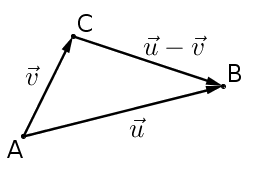
\includegraphics[width=4.5cm]{def.png}}

\dleft{12cm}{
\begin{propriete}[ - Avec des normes seulement (2)]
    $$\vv{u} \cdot \vv{v} =\dfrac{1}{2}\left( \left\|\vv{u}+\vv{v}\right\|^2 - \left\|\vv{u}\right\|^2 - \left\|\vv{v}\right\|^2 \right)$$ 
\end{propriete}}
{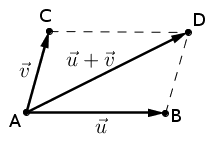
\includegraphics[width=4.5cm]{prop1.png}}


\begin{propriete}[ - Avec le projeté orthogonal]
    Soit $H$ le projeté orthogonal de $C$ sur la droite $(AB)$.
    \begin{tabbing}
        $\vv{AB} \cdot \vv{AC}$ \= $=\vv{AB} \cdot \vv{AH}$\\
        \>$=\left\{\begin{array}{ll}
			AB\times AH & \text{si } \vv{AB} \text{ et } \vv{AH} \text{ sont de même sens} \\
			-AB\times AH & \text{si } \vv{AB} \text{ et } \vv{AH} \text{ sont de sens opposés} \\
		\end{array}
		\right.$ 
    \end{tabbing}
   
    \begin{multicols}{2}
        \begin{tikzpicture}[scale=1]
  % Origine
  \coordinate (A) at (0,0);
  % Vecteur u
  \coordinate (U) at (3,0);
  % Vecteur v
  \coordinate (V) at (2,2);
  % Proj de v sur u
  \coordinate (P) at (2,0);

  % Vecteur u
  \draw[->, thick, UGLiBlue] (A) -- (U) node[below right] {$B$};
  % Vecteur v
  \draw[->, thick, UGLiRed] (A) -- (V) node[above] {$C$};
  % Proj de v sur u
  \draw[dashed] (V) -- (P);
  %\draw[fill=black] (P) circle (0.04);
  \node[below] at (P) {$H$};
  % Angle
  \draw (0.6,0) arc (0:45:0.6);
  \node at (0.8,0.25) {$\theta$};
  % Codage angle droit
  \draw (P) ++(-0.2,0) -- ++(0,0.2) -- ++(0.2,0);
  % Point O
  \fill (A) circle (0.04);
  \node[below left] at (A) {$A$};
\end{tikzpicture}

        \begin{tikzpicture}[scale=1]
  % Origine
  \coordinate (A) at (0,0);
  % Vecteur u
  \coordinate (U) at (3,0);
  % Vecteur v (angle obtus)
  \coordinate (V) at (-1,2);
  % Proj de v sur u 
  \coordinate (P) at (0,0); 
  \coordinate (H) at (-1,0);

  % Vecteur u
  \draw[->, thick, UGLiBlue] (A) -- (U) node[below right] {$B$};
  % Vecteur v
  \draw[->, thick, UGLiRed] (A) -- (V) node[above left] {$C$};
  % Proj de v sur u (ici, sur O)
  \draw[dashed] (V) -- (H);
  \draw[dashed] (-2,0) -- (P);
  \draw[fill=black] (P) circle (0.04);
  \node[below] at (H) {$H$};
  % Angle obtus
  \draw (0.6,0) arc (0:116.5:0.6);
  \node[above right] at (0.2,0.5) {$\theta$};
  % Codage angle droit
  \draw (H) ++(-0.2,0) -- ++(0,0.2) -- ++(0.2,0);
  % Point O
  \fill (A) circle (0.04);
  \node[below left] at (A) {$A$};
\end{tikzpicture}
    \end{multicols}
\end{propriete}

\begin{propriete}[ - Avec les coordonnées]
    Si, on a : $\vc{u}{x}{y}$ et $\vc{v}{x'}{y'}$, alors : $$\vv{u} \cdot \vv{v} = x x' + y y'.$$
\end{propriete}
   
\begin{propriete}[ - Avec un angle]
    $$\vv{AB} \cdot \vv{AC} = AB \times AC \times \cos(\theta)$$
    \begin{multicols}{2}
        \begin{tikzpicture}[scale=1]
  % Origine
  \coordinate (A) at (0,0);
  % Vecteur u
  \coordinate (U) at (3,0);
  % Vecteur v
  \coordinate (V) at (2,2);
  % Proj de v sur u
  \coordinate (P) at (2,0);

  % Vecteur u
  \draw[->, thick, UGLiBlue] (A) -- (U) node[below right] {$B$};
  % Vecteur v
  \draw[->, thick, UGLiRed] (A) -- (V) node[above] {$C$};
 
  % Angle
  \draw (0.6,0) arc (0:45:0.6);
  \node at (0.8,0.25) {$\theta$};
  
  % Point O
  \fill (A) circle (0.04);
  \node[below left] at (A) {$A$};
\end{tikzpicture}

        \begin{tikzpicture}[scale=1]
  % Origine
  \coordinate (A) at (0,0);
  % Vecteur u
  \coordinate (U) at (3,0);
  % Vecteur v (angle obtus)
  \coordinate (V) at (-1,2);
  % Proj de v sur u 
  \coordinate (P) at (0,0); 
  \coordinate (H) at (-1,0);

  % Vecteur u
  \draw[->, thick, UGLiBlue] (A) -- (U) node[below right] {$B$};
  % Vecteur v
  \draw[->, thick, UGLiRed] (A) -- (V) node[above left] {$C$};
  
  % Angle obtus
  \draw (0.6,0) arc (0:116.5:0.6);
  \node[above right] at (0.2,0.5) {$\theta$};
  
  % Point O
  \fill (A) circle (0.04);
  \node[below left] at (A) {$A$};
\end{tikzpicture}
    \end{multicols}
\end{propriete}


\begin{exemple}[ 1]
        \dleft{10cm}{
        \begin{tabbing}
            $\vv{AB} \cdot \vv{AC}$ \= $=\vv{AB} \cdot \vv{AH}$\\
            \> $=AB \times AH$\\
            \> $=6 \times 4$\\
            \> $=24$
        \end{tabbing}}
        {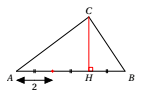
\includegraphics[width=4.5cm]{exemple1.png}}
\end{exemple}

\begin{exemple}[ 2]
    \dleft{10cm}{
    \begin{tabbing}
        $\vv{u} \cdot \vv{v}$ \= $=4 \times 1 + 2 \times 2$\\
        \> $=8$
    \end{tabbing}}
    {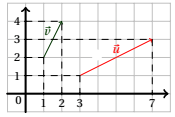
\includegraphics[width=5cm]{exemple2.png}}
\end{exemple}

\begin{exemple}[ 3]
    \dleft{10cm}{
    \begin{tabbing}
        $\vv{AB} \cdot \vv{AC}$ \= $=AB \times AC \times \cos(\widehat{BAC})$\\
        \> $=2\times 2\times \cos\left(\dfrac{2\pi}{3}\right)$\\
        \> $=-2$
    \end{tabbing}}
    {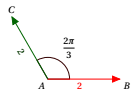
\includegraphics[width=4cm]{exemple3.png}}
\end{exemple}

\begin{exemple}[ 4]
    \dleft{10cm}{
    \begin{tabbing}
        $\vv{AB} \cdot \vv{AC}$ \= $=\dfrac{1}{2}\left(\left\|\vv{AB}\right\|^2+\left\|\vv{AC}\right\|^2-\left\|\vv{AB}-\vv{AC}\right\|^2\right)$\\[.5em]
        \> $=\dfrac{1}{2}\left(AB^2+AC^2-CB^2\right)$\\[.5em]
        \> $=\dfrac{1}{2}\left(4^2+6^2-3^2\right)$\\[.5em]
        \> $=\dfrac{43}{2}$
    \end{tabbing}}
    {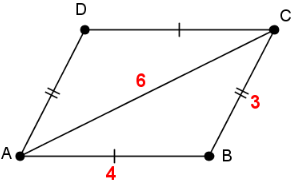
\includegraphics[width=4.5cm]{exemple4.png}}
\end{exemple}

\begin{remarque}[ : Cas particuliers]
    \begin{enumerate}[label=\textbullet]
        \item $\vv{u} \cdot \vv{u} = \left\|\vv{u}\right\|^2$.\\
        $\vv{u} \cdot \vv{u}$ se note aussi $\vv{u}^2$.
        \item Si $\vv{u}$ et $\vv{v}$ sont colinéaires, alors \\[.5em]
            $\vv{u} \cdot \vv{v}=\left\{\begin{array}{ll}
			\left\| \vv{u}\right\|\times \left\|\vv{v}\right\| & \text{si } \vv{u} \text{ et } \vv{v} \text{ sont de même sens} \\
			-\left\| \vv{u}\right\|\times \left\|\vv{v}\right\| & \text{si } \vv{u} \text{ et } \vv{v} \text{ sont de sens opposés.} \\
		\end{array}
		\right.$ 
    \end{enumerate}
\end{remarque}

\begin{exemple}[ 5]
    \dleft{8cm}{
    On a :
    \begin{tabbing}
        $\vv{AB} \cdot \vv{AB}$ \= $=\left\|\vv{AB}\right\|^2$\\
        \>$=9$
    \end{tabbing}
    On peut également écrire $\vv{AB}^2 = 9$.\\[.5em]
    On a aussi :
    \begin{tabbing}
        $\vv{AB} \cdot \vv{AC}$ \= $=-\left\|\vv{AB}\right\|\times \left\|\vv{AC}\right\|$\\
        \> $=-3\times 2$\\
        \> $=-6$
    \end{tabbing}}
    {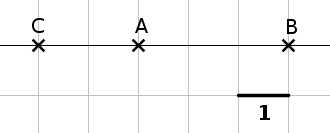
\includegraphics[width=5cm]{exemple5.png}}
\end{exemple}

\section{Propriétés du produit scalaire}
\begin{propriete}[s]
    Soient $\vv{u}$, $\vv{v}$ et $\vv{w}$ trois vecteurs et $k$ un réel.
    \begin{enumerate}[label=\textbullet]
        \item \textbf{symétrie} : $\vv{u} \cdot \vv{v} = \vv{v} \cdot \vv{u}$.
        \item \begin{tabbing}
            \textbf{linéarité} :  \=$\left(k\vv{u}\right) \cdot \vv{v} = k\left(\vv{u} \cdot \vv{v}\right)$\\
            \> $\vv{u} \cdot \left(\vv{v}+ \vv{w}\right) = \vv{u} \cdot \vv{v}+\vv{u}\cdot \vv{w}$\\
        \end{tabbing}
    \end{enumerate}
\end{propriete}

\begin{propriete}[ - Identités remarquables]
    Soient $\vv{u}$ et $\vv{v}$ deux vecteurs.
    \begin{enumerate}[label=\textbullet]
        \item $\left(\vv{u}+\vv{v}\right)^2 = \vv{u}^2  + 2\vv{u} \cdot \vv{v}+ \vv{v}^2$
        \item $\left(\vv{u}-\vv{v}\right)^2 = \vv{u}^2  - 2\vv{u} \cdot \vv{v}+ \vv{v}^2$
        \item $\left(\vv{u}+\vv{v}\right) \cdot \left(\vv{u}-\vv{v}\right) = \vv{u}^2 - \vv{v}^2$
    \end{enumerate}
\end{propriete}

\begin{demonstration}[ (du point 2)]
    \begin{tabbing}
        $\left(\vv{u}-\vv{v}\right)^2$ \= $=\left(\vv{u}-\vv{v}\right) \cdot \left(\vv{u}-\vv{v}\right)$\\
        \> $=\left(\vv{u} \cdot \vv{u}\right) - \left(\vv{u} \cdot \vv{v}\right) - \left(\vv{v} \cdot \vv{u}\right) + \left(\vv{v} \cdot \vv{v}\right)$\\
        \> $=\vv{u}^2 - 2\vv{u} \cdot \vv{v}  + \vv{v}^2$
    \end{tabbing}
\end{demonstration}

\section{Vecteurs orthogonaux}
\begin{definition}[]
    Deux vecteurs non nuls $\vv{AB}$ et $\vv{CD}$ sont dits \textbf{orthogonaux} si les droites $(AB)$ et $(CD)$ sont perpendiculaires.
\end{definition}

\begin{remarque}[]
    Par convention, on dit que le vecteur nul $\vv{0}$ est orthogonal à tout vecteur.
\end{remarque}

\begin{propriete}[]
    Deux vecteurs sont orthogonaux si, et seulement si, leur produit scalaire est nul.
\end{propriete}

\begin{exemple}[]
    Les droites $(CA)$ et $(CB)$ sont-elles perpendiculaires ?
    \begin{center}
        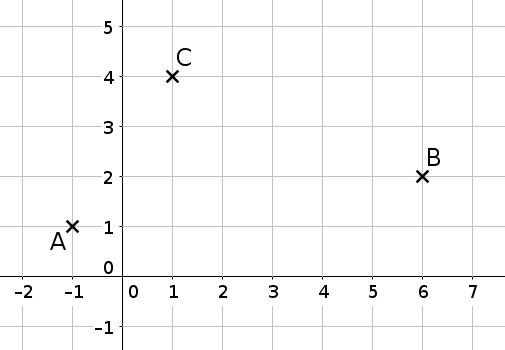
\includegraphics[width=7cm]{exemple6.png}
    \end{center}
    On a : $\vc{CA}{1}{-2}$ et $\vc{CB}{4}{2}$.\\[.5em]
    On calcule le produit scalaire :
    \begin{tabbing}
        $\vv{CA} \cdot \vv{CB}$ \= $=1\times 4 + (-2)\times 2$\\
        \> $=4 - 4$\\
        \> $=0$
    \end{tabbing}
    Donc, les vecteurs $\vv{CA}$ et $\vv{CB}$ sont orthogonaux, c'est-à-dire que les
    droites $(CA)$ et $(CB)$ sont perpendiculaires.
\end{exemple}
\end{document}